\documentclass[
  aspectratio=169,
  %aspectratio=43,
]{beamer}

\usepackage[english]{babel}
\usepackage[utf8]{inputenc}
\usepackage[T1]{fontenc}
\usepackage{booktabs}
\usepackage{listings}

\usetheme[
  workplace=rect,
]{MU}
\begin{document}

\title[STM32 Nucleo-F411RE Board Support Crate]{STM32 Nucleo-F411RE \\Board Support Crate for Embedded Rust}
\subtitle[Short Presentation Subtitle]{D7018E - Special Studies in Embedded Systems}
\author[J.\,Sjölund]{Johannes Sjölund \\ johsjl-1@student.ltu.se}
\institute[LTU]{Luleå University of Technology}
\date{\today}
\subject{STM32 Nucleo-F411RE Board Support Crate for Embedded Rust}
\keywords{the, presentation, keywords}

\begin{frame}[plain]
\maketitle
\end{frame}

%\begin{frame}{Table of Contents}
%\tableofcontents
%\end{frame}

%\section[Short Section 1 Name]{Full Section 1 Name}
%\subsection[Short Subsection 1 Name]{Full Subsection 1 Name}

\begin{frame}{STM32 Nucleo-F411RE}
\begin{columns}[T] % align columns
\hfill%

\begin{column}{.5\textwidth}
\begin{itemize}
\item Development board for the Arm Cortex-M4 microcontroller STM32F411RE by STMicroelectronics. 
\item Supports Arduino header expansion boards, as well as STM32 Nucleo Morpho headers.
\item Power, buttons, LEDs, programmer IC, USB-to-Serial converter.
\end{itemize}
\end{column}%
\hfill%
\begin{column}{.6\textwidth}
\vspace{-22mm}
\begin{figure}
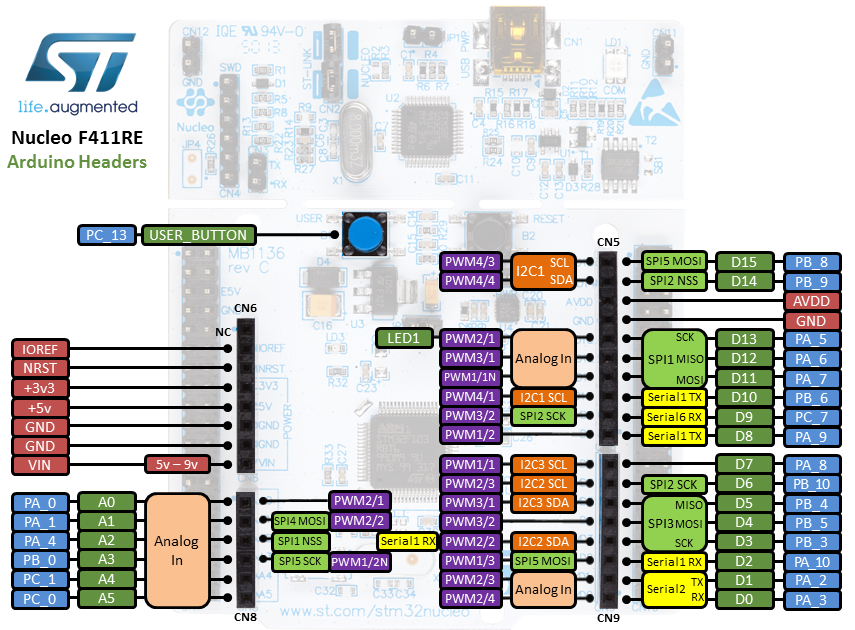
\includegraphics[width=.9\textwidth,height=.9\textheight,keepaspectratio]{Nucleo_f411re.png}
\caption{Map of hardware peripheral resources on the Nucleo-F411RE.}
\end{figure}
\end{column}%
\end{columns}
\footnote{http://www.st.com/en/evaluation-tools/nucleo-f411re.html}
\end{frame}

\begin{frame}{Real-time systems programming}{}
\begin{columns}[T] % align columns
\hfill%
\begin{column}{.5\textwidth}
Our programs must:
\begin{enumerate}
  \item Respond to many different external events, all in a timely fashion and never miss anything.
	\begin{itemize}
	  \item Button clicks
	  \item Communication
	  \item The passing of time
	\end{itemize}
  \item Be correct and never enter an undefined state.
  \item Not waste power.
\end{enumerate}
\end{column}%
\hfill%
\begin{column}{.5\textwidth}
\emph{Problem:}

How does a real-time system read and write mutable resources when different processes can access them at any time?
\begin{itemize}
  \item \alert{Data race} conditions can be solved by mutual exclusion on critical sections.
  \item Mutual exclusion can lead to \alert{deadlock} if system uses resource holding, circular wait and no preemption.
\end{itemize}
\end{column}%
\end{columns}
\end{frame}

\begin{frame}{RTFM}{Real-Time For the Masses (RTFM)}
Programming model for robust real-time systems. \footnote{P Lindgren, M Lindner, A Lindner. \structure{RTFM-core: Language and Implementation.} LTU, 2015}
\begin{itemize}
  \item Based on a reactive programming model involving \alert{tasks} and \alert{resources}.
  \item Resource management provided by the \alert{Stack Resource Policy} (SRP).
  \item Uses the underlying interrupt hardware for static priority scheduling of tasks (the \texttt{BASEPRI} register).
  \item Guarantees \alert{deadlock-lock free} execution.
\end{itemize}
\end{frame}

\begin{frame}{Rust}{What is special about it?}
\begin{columns}[T] % align columns
\begin{column}{.8\textwidth}
Designed for highly concurrent and highly safe systems, in the context of memory safety.
\begin{itemize}
  \item Does not permit \alert{dangling pointers}, or \alert{data races} in safe code.
  \item Unsafe code can still be used, but must be tagged as \texttt{unsafe\{\}}.
\end{itemize}
Does not perform automated \alert{garbage collection} like Go, Java or .NET, where resources like heap memory used by unused variables are freed periodically. Rust frees them when variables gets out of scope according to its \structure{ownership} and \structure{borrowing} system. 
\end{column}%
\begin{column}{.2\textwidth}
\vspace{-0mm}
\begin{figure}
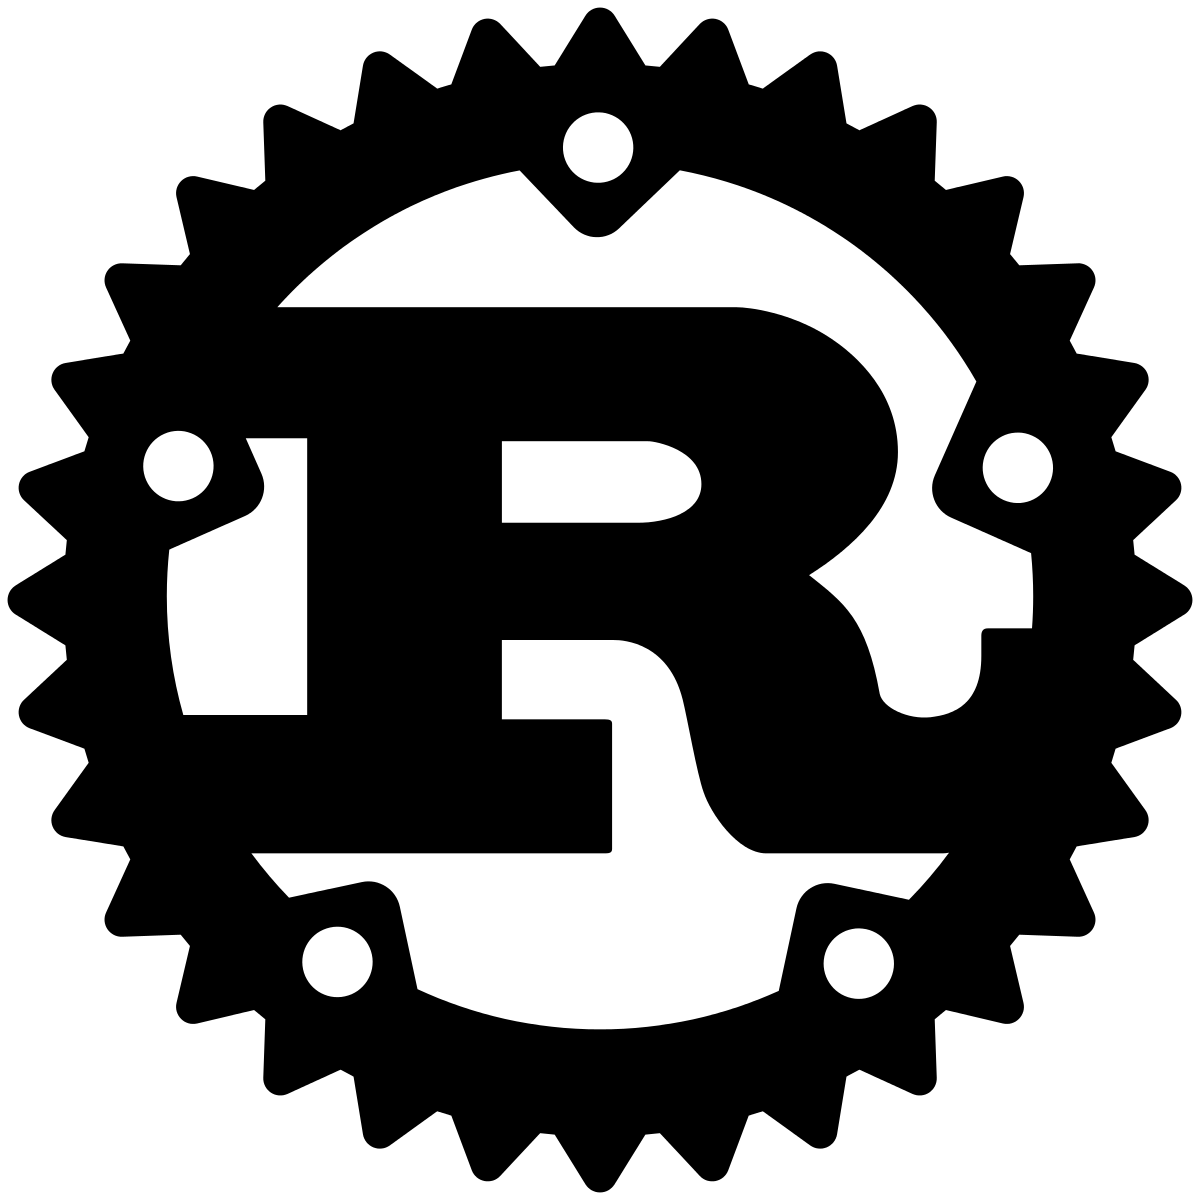
\includegraphics[width=1\textwidth,height=1\textheight,keepaspectratio]{rust.png}
\end{figure}
\end{column}%
\end{columns}
\footnote{\url{https://www.rust-lang.org/en-US/}}
\end{frame}



\begin{frame}[fragile]{cortex-m-rtfm}{Rust crate for RTFM on Arm Cortex-M}
Rust crate (code library) which combines the best of Rust and RTFM, written by \\Jorge Aparicio and Per Lindgren.

\vspace{2mm}

Designed around a concept of \structure{tasks} and \structure{resources}, where tasks 
\begin{itemize}
  \item are \alert{event triggered},
  \item are assigned \alert{constant priorities},
  \item must not contain endless loops. \footnote{\url{https://docs.rs/cortex-m-rtfm/0.3.1/cortex_m_rtfm/}}
\end{itemize}
\end{frame}


\begin{frame}{Programming embedded Rust}{}
The \structure{cortex-m-rtfm} crate is great, but how to make use of it for a specific microcontroller? 

\vspace{2mm}

Manufacturers like STMicroelectronics and NXP Semiconductors provide \alert{SVD files} (XML) which describes the hardware features, memory layout, and register functions of the device.

\vspace{2mm}

The SVD file can be used by \alert{svd2rust}\footnote{\url{https://docs.rs/svd2rust/0.12.0/svd2rust/}} to generate Rust code for peripheral access on the microcontroller.

\vspace{2mm}

\url{https://gitlab.henriktjader.com/pln/STM32F40x}

\end{frame}

\begin{frame}{Board support crates}{}
We can use the code from \alert{svd2rust} to access the microcontroller registers, but how do we know what to do with them? What is \texttt{stm32f40x::dma2::s0ndtr::ndt}?

\vspace{2mm}

Read the \alert{datasheet} \footnote{\url{http://www.st.com/resource/en/datasheet/stm32f411re.pdf}} and \alert{reference manual} \footnote{\url{http://www.st.com/resource/en/reference_manual/dm00119316.pdf}}.

\vspace{2mm}

To speed up development, a board support crate can provide a hardware abstraction layer, and examples of how to use the devices.

\begin{itemize}
  \item STM32F3DISCOVERY: \url{https://github.com/japaric/f3}
  \item Blue-pill: \url{https://github.com/japaric/blue-pill}
  \item \alert{Nucleo-F411RE}: \url{https://github.com/jsjolund/f4}
\end{itemize}
\end{frame}


\begin{frame}{STM32 Nucleo-F411RE Board Support Crate}
\begin{columns}[T] % align columns
\hfill%
\begin{column}{.53\textwidth}
\vspace{-2mm}
Provides an abstraction layer for STM32F40x
\begin{itemize}
\item GPIO
\item ADC
\item Communication
	\begin{itemize}
	\item I$^2$C, SPI
	\item UART (serial) over USB using ST-Link-v2
	\end{itemize}
\item Timers
	\begin{itemize}
	\item Microsecond counter
	\item PWM generation
	\item Input capture
	\end{itemize}
\item DMA
\item Clocking (16-100 MHz)
\end{itemize}
\end{column}%
\hfill%
\begin{column}{.47\textwidth}
\vspace{-5mm}
\begin{figure}
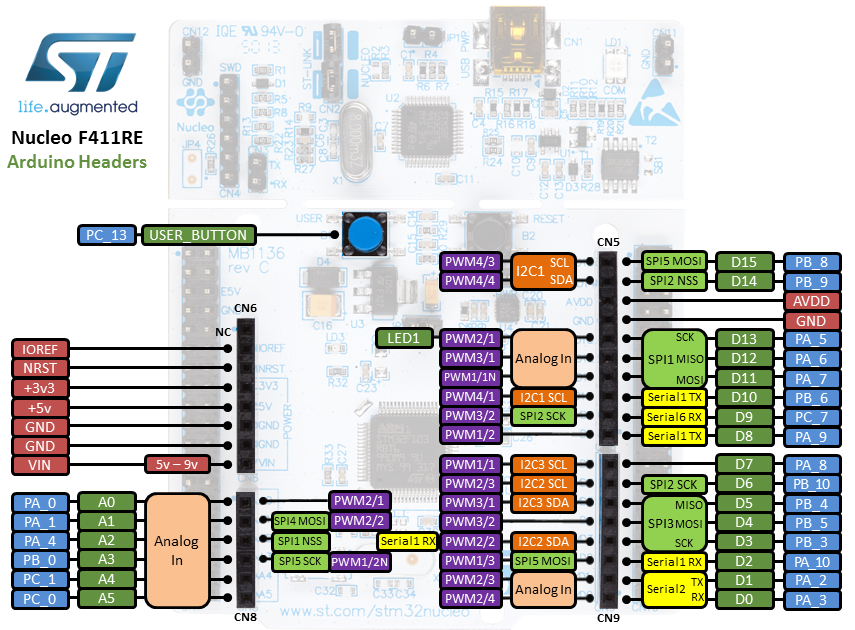
\includegraphics[width=1.03\textwidth,height=1.03\textheight,keepaspectratio]{Nucleo_f411re.png}
%\caption{Map of hardware peripheral resources on the Nucleo-F411RE.}
\end{figure}
\end{column}%
\end{columns}

\end{frame}


\begin{frame}{Usage /examples/imu.rs}
\begin{columns}[T] % align columns
\hfill%
\begin{column}{.53\textwidth}
\vspace{-2mm}
The inertial measurement unit LSM9DS1 can communicate through SPI and report
\begin{itemize}
\item Acceleration (accelerometer)
\item Rotational velocity (gyro)
\item Magnetic field strength (magnetometer)
\end{itemize}
Sensor fusion algorithms such as \alert{Madgwick AHRS} can take these measurements and calculate current attitude/orientation relative to Earth's horizontal plane.
\end{column}%
\hfill%
\begin{column}{.47\textwidth}
\vspace{-10mm}
\begin{figure}
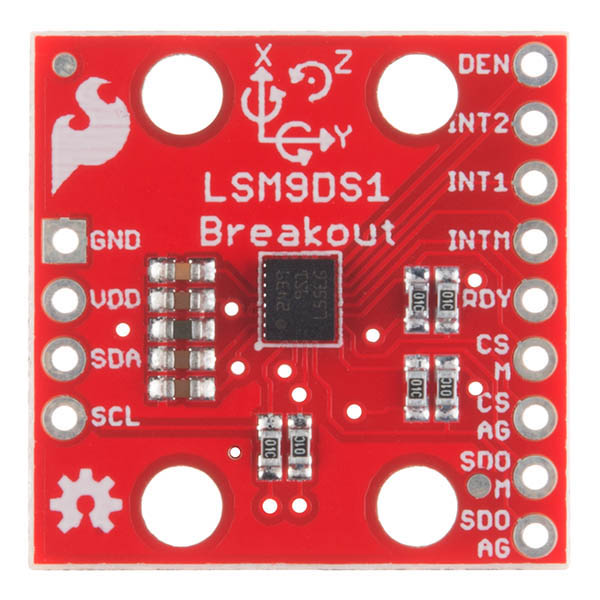
\includegraphics[width=0.8\textwidth,height=0.8\textheight,keepaspectratio]{lsm9ds1.jpg}
%\caption{Map of hardware peripheral resources on the Nucleo-F411RE.}
\end{figure}
\end{column}%
\end{columns}
\footnote{http://x-io.co.uk/open-source-imu-and-ahrs-algorithms/}
\end{frame}

\begin{frame}{Usage /examples/eeprom.rs}
\begin{columns}[T] % align columns
\hfill%
\begin{column}{.53\textwidth}
\vspace{10mm}
To store persistent data such as user settings, we may want to use an external EEPROM. The Microchip 24LC64 can communicate through the I$^2$C protocol for reading and writing.
\end{column}%
\hfill%
\begin{column}{.47\textwidth}
\vspace{-10mm}
\begin{figure}
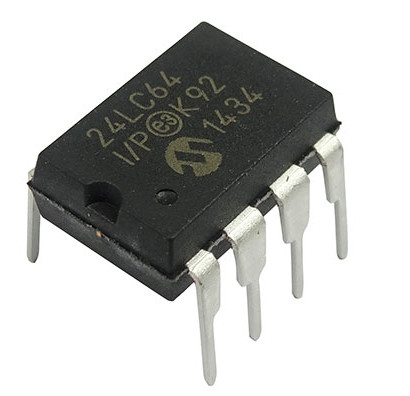
\includegraphics[width=0.8\textwidth,height=0.8\textheight,keepaspectratio]{24lc64.jpg}
%\caption{Map of hardware peripheral resources on the Nucleo-F411RE.}
\end{figure}
\end{column}%
\end{columns}
\end{frame}



\begin{frame}{Other examples}
\begin{itemize}
\item \structure{/examples/adc1.rs} - Reading ADC using a timer and DMA.
\item \structure{/examples/usart2-dma.rs} - Serial communication over USB using DMA.
\item \structure{/examples/button.rs} - Toggling the LED when user interrupts with button.
\item \structure{/examples/pwm1.rs} - Output PWM signal using timer.
\item \structure{/examples/capture4.rs} - Measure PWM signal frequency using timer.
\end{itemize}
\end{frame}



\begin{frame}{Limitations/Future work}
\begin{itemize}
\item Different peripheral \alert{pin mappings} are available but not supported.
\item Should be converted to the \alert{singletons} framework.
\item Add features like
	\begin{itemize}
	\item Timer encoder support,
	\item Injected mode ADC,
	\item Real-time clock,
	\item USB OTG,
	\item Secure digital card support,
	\item More DMA.
	\end{itemize}
\item Lots and lots of \alert{usability} improvements.
\end{itemize}
\end{frame}



\begin{frame}{Questions?}
Bug reports and pull requests are always welcome.
\end{frame}

\end{document}
